%% Start of file `dndicons-doc.tex`.
%% Copyright 2024 Jasper Habicht (mail@jasperhabicht.de).
%
% This work may be distributed and/or modified under the
% conditions of the LaTeX Project Public License version 1.3c,
% available at http://www.latex-project.org/lppl/.

\documentclass[a4paper]{article}
\def\dndiconsfileversion{1.5.5}
\def\dndiconsfiledate{7 March 2024}

\usepackage[T1]{fontenc}
\usepackage{Alegreya}
\usepackage{AlegreyaSans}
\usepackage{FiraMono}

\usepackage{geometry, longtable, booktabs, tcolorbox, hyperref}
\geometry{margin=25mm, left=45mm}

\usepackage{fancyhdr}
\pagestyle{fancy}
\fancyhf{}
\renewcommand{\headrulewidth}{0pt}
\fancyfoot[R]{\thepage}

\linespread{1.1}\selectfont
\addtolength{\skip\footins}{1em plus 5pt}
\makeatletter
\renewcommand*{\thefootnote}{\fnsymbol{footnote}}
\renewcommand{\@makefntext}[1]{%
    \noindent\hbox to 0.75em{\normalfont\@thefnmark\hss}~#1%
}
\makeatother

\tcbuselibrary{listings}
\lstdefinestyle{dndiconsdocmacro}{
    basicstyle=\small\ttfamily,
    literate=*{<}{{{\color{black!50}\guilsinglleft}}}1 
        {>}{{{\color{black!50}\guilsinglright}}}1,
    keywords={},
    moredelim=[is][\bfseries]{|}{|},
    moredelim=[is][\color{black!50}]{!}{!},
}
\lstdefinestyle{dndiconsdoccodeexample}{
    basicstyle=\small\ttfamily,
    keywords={},
}

\hypersetup{colorlinks}

\ExplSyntaxOn
\int_new:N \l_dndicons_doc_change_int
\NewDocumentCommand{\changes}{ m m m }{
    \int_incr:N \l_dndicons_doc_change_int
    \prop_new:c { l_dndicons_doc_change_ 
        \int_to_roman:n { \l_dndicons_doc_change_int } _prop }
    \prop_put:cnn { l_dndicons_doc_change_ 
        \int_to_roman:n { \l_dndicons_doc_change_int } _prop } { version } {#1}
    \prop_put:cnn { l_dndicons_doc_change_ 
        \int_to_roman:n { \l_dndicons_doc_change_int } _prop } { date } {#2}
    \prop_put:cnn { l_dndicons_doc_change_ 
        \int_to_roman:n { \l_dndicons_doc_change_int } _prop } { changes } {#3}
}
\NewDocumentCommand{\printchanges}{ }{
    \section{Changes}
    \begin{description}
    \int_step_inline:nn { \l_dndicons_doc_change_int } {
        \item[ 
            \prop_item:cn { l_dndicons_doc_change_ 
            \int_to_roman:n { ##1 } _prop } { version } ] 
            ( \prop_item:cn { l_dndicons_doc_change_ 
            \int_to_roman:n { ##1 } _prop } { date } ) \\
            \prop_item:cn { l_dndicons_doc_change_ 
            \int_to_roman:n { ##1 } _prop } { changes }
    }
    \end{description}
}

\tl_new:N \l_dndicons_doc_doctitle_tl
\NewExpandableDocumentCommand{\makedoctitle}{ o m o m m o m }{
    \hypersetup{
        pdfauthor={#5},
        pdftitle={\IfValueTF{#1}{#1}{#2}},
        pdfsubject={\IfValueTF{#3}{#3}{#4}}
    }
    \tl_set:Nn \l_dndicons_doc_doctitle_tl {
        \group_begin:
            \tcbset{
                title ~ style ~ hook/.style={
                    boxrule=2pt,
                    fontupper=\huge\ttfamily
                }
            }
            \setlength{\parindent}{0pt}\sffamily
            \Huge{\bfseries #2}\par\bigskip
            \Large #4\par\bigskip
            \large #5
            \IfValueT{#6}{
                \,\footnote{#6}\par\bigskip
            }
            #7\par\bigskip
            \rule{\textwidth}{.08em}
        \group_end:
    }
}

\NewExpandableDocumentCommand{\printdoctitle}{ }{
    \tl_use:N \l_dndicons_doc_doctitle_tl
}
\ExplSyntaxOff

\tcbset{
    size=small,
    arc=2.5pt,
    outer arc=2.5pt,
    colframe=black!10,
    colback=black!10,
    title style hook/.style={}
}

\NewTCBListing{macrodef}{ }{ 
    listing only,
    listing style={dndiconsdocmacro},
    grow to left by=2cm,
    boxrule=0pt,
    after={\par\smallskip\noindent}
}

\NewTCBListing{codeexample}{ }{
    text side listing,
    lefthand width=4.5cm,
    listing style={dndiconsdoccodeexample},
    after={\par\smallskip\noindent}
}

\NewTotalTCBox{\macro}{ O{} v }{
    verbatim,
    size=tight,
    arc=1pt,
    outer arc=1pt,
    top=0.5pt, 
    bottom=0.5pt,
    left=2pt, 
    right=2pt,
    boxrule=0pt,
    colframe=black!10,
    colback=black!10,
    fontupper=\small\ttfamily,
    #1
}{\vphantom{/g}\lstinline^#2^}

\NewTotalTCBox{\titlemacro}{ s O{} m }{
    verbatim,
    size=tight,
    arc=1pt,
    outer arc=1pt,
    top=0.5pt, 
    bottom=0.5pt,
    left=2pt, 
    right=2pt,
    boxrule=0pt,
    colframe=black!10,
    colback=black!10,
    fontupper=\small\ttfamily,
    title style hook,
    #2
}{\vphantom{/g}\IfBooleanT{#1}{\textbackslash}#3}

\usepackage[pics]{dndicons}
\usepackage{dndicons-l3draw}

\ExplSyntaxOn
\clist_new:N \l_dndicons_doc_logo_icons_clist
\clist_new:N \l_dndicons_doc_logo_colors_clist
\cs_generate_variant:Nn { \color_set:nnn } { nne }

\clist_set:Nn \l_dndicons_doc_logo_colors_clist { 
    264653 , 287271 , 2a9d8f , e9c46a , f4a261 , e76f51 
}
\int_step_inline:nn { \clist_count:N \l_dndicons_doc_logo_colors_clist } {
    \color_set:nne { dndiconslogo \int_to_roman:n { #1 } } { HTML } {
        \clist_item:Nn \l_dndicons_doc_logo_colors_clist { #1 }
    }
}
\clist_set:Nn \l_dndicons_doc_logo_icons_clist { 
    twentyside , charisma , armor , buff , ranged , proficiency 
}

\NewDocumentCommand{\dndiconslogo}{ O{1} }{
    \draw_begin:
        \draw_transform_scale:n { #1 }
        \int_step_inline:nn { \clist_count:N \l_dndicons_doc_logo_icons_clist } {
            \hcoffin_set:Nn \l_tmpa_coffin { 
                \draw_suspend_begin: 
                    \DndiconsAbility[negative]{ 
                        \clist_item:Nn \l_dndicons_doc_logo_icons_clist { ##1 } 
                    }[color=dndiconslogo \int_to_roman:n { ##1 } ] 
                \draw_suspend_end: 
            }
            \draw_scope_begin:
                \draw_transform_shift:n { 
                    % fix bug in older l3draw version
                    \cs_if_exist:NTF \__draw_transform_shift:nnnn { 
                        \draw_point_polar:nn { 0.33cm } { 60 * ##1 + 10 }
                    } {
                        \draw_point_transform:n { \draw_point_polar:nn { 0.33cm } { 60 * ##1 + 10 } }
                    }
                }
                \draw_coffin_use:Nnn \l_tmpa_coffin { hc } { vc } 
            \draw_scope_end:
        }
    \draw_end:
}
\ExplSyntaxOff

\NewDocumentEnvironment{dndiconsiconlist}{ }{
    \begin{longtable}{ @{} p{20em} p{5em} p{\dimexpr\linewidth-25em-4\tabcolsep} @{} }
    \toprule
    \textbf{Command} & \textbf{Icon} & \textbf{Shape} \\ 
    \midrule\endhead
}{
    \bottomrule
    \end{longtable}
}

\makedoctitle
    [The dndicons package]
    {The \titlemacro{dndicons} package}
    {A set of high-quality icons made with Ti\emph{k}Z for use in notes for tabletop role-playing games}
    {Jasper Habicht}[E-mail: \href{mailto:mail@jasperhabicht.de}{mail@jasperhabicht.de}]
    {Version \dndiconsfileversion, released on \dndiconsfiledate}

\changes{v1.1.0}{2023/08/15}{First public release.}
\changes{v1.1.1}{2023/11/15}{Fudge dice icon added.}
\changes{v1.1.2}{2023/11/16}{Bug fixed that caused wrong spacing when using dice icons without quantifier.}
\changes{v1.2.0}{2023/11/20}{Corrections in the manual. Icons for six-sided dice with one to nine pips, plus sign and minus sign added.}
\changes{v1.2.1}{2023/11/20}{Documentation of lengths for spacing added.}
\changes{v1.2.2}{2023/11/21}{Corrections in the manual.}
\changes{v1.3.0}{2023/11/21}{Option to set background color added. Renamed global option.}
\changes{v1.3.1}{2024/02/18}{Correction of initializing code. Correction of default value of after sep. Addition of pics.}
\changes{v1.3.2}{2024/02/19}{Reformatting of the manual.}
\changes{v1.3.4}{2024/02/20}{Minor corrections of some shapes.}
\changes{v1.4.0}{2024/02/21}{\titlemacro{l3draw} variant added.}
\changes{v1.4.1}{2024/02/21}{Corrections in \titlemacro{l3draw} variant.}
\changes{v1.4.2}{2024/02/21}{Alternative set of commands in \titlemacro{l3draw} variant defined.}
\changes{v1.4.3}{2024/02/22}{Added option to \titlemacro{l3draw} variant to enable upward compatibility.}
\changes{v1.4.4}{2024/02/24}{Added styles for every instance of command or shape, correction of recent \titlemacro{l3draw} code.}
\changes{v1.5.0}{2024/02/25}{Alternative set of commands defined, added support of styles in pics.}
\changes{v1.5.1}{2024/02/28}{Addition of opacity to \titlemacro{l3draw} variant.}
\changes{v1.5.2}{2024/02/29}{Unification of scaling, minor corrections.}
\changes{v1.5.3}{2024/03/03}{Optimisation of code in \titlemacro{l3draw} variant.}
\changes{v1.5.4}{2024/03/06}{Correction of baseline settings in \titlemacro{l3draw} variant, added accessibililty support for \titlemacro{l3draw} variant.}
\changes{v1.5.5}{2024/03/07}{Optimsation of accessibililty support for \titlemacro{l3draw} variant.}

\begin{document}

\vspace*{-1cm}
\noindent\dndiconslogo[4]

\bigskip

\printdoctitle

\bigskip

\section{Introduction}

The \macro{dndicons} package provides a set of high-quality icons made with Ti\emph{k}Z for use in notes for tabletop role-playing games. The icons are meant to be used in the body text, but they can also be used in other contexts such as graphics or diagrams.

Since the commands to typeset the icons use \macro{tikzpicture} environments, these commands should not be used inside another \macro{tikzpicture}. However, because the package defines the icons as Ti\emph{k}Z shapes, it is possible to use the icons in \macro{tikzpicture} environments directly. 

Apart from that, as of version 1.1.0, the package provides a way to define custom commands to typeset the icons as boxed material which is safe to use in a \macro{tikzpicture} context. As of version 1.3.1, the package provides an additional way to use the icons as Ti\emph{k}Z pics. As of version 1.4.0, a variant of the package provides an alternative way to typeset the icons using the \macro{l3draw} packagee.

\section{Loading the package}

The package can be installed by copying the file \macro{dndicons.sty} into the working directory or into the \macro{texmf} directory. After the package has been installted, the \macro{dndicons} package is loaded by calling \macro{\usepackage{dndicons}} in the preamble of the document. 

\begin{macrodef}pics\end{macrodef}
The package provides the option \macro{pics}. If the package is loaded with this option, every icon is also available as Ti\emph{k}Z pic. On the use of pics, see section \ref{sec:pics} below.

\subsection{Dependencies}

The package loads the \macro{tikz} package which in turn loads the \macro{xcolor} package. If you want to make use of certain options these packages provide, you need to load the packages with the relevant options beforehand or use, for example, \macro{\PassOptionsToPackage{svgnames}{xcolor}}.

\section{Usage}

Once loaded, the package provides a set of commands that can be used to print icons inline. The package also defines a set of node shapes that can be used inside a \macro{tikzpicture} environment. 

\subsection{Global settings}

\begin{macrodef}dnd icons\end{macrodef}
All icons share the Ti\emph{k}Z style \macro{dnd icons} that has no options per default but can be used to style all icons at once. For example, if \macro{\tikzset{dnd icons/.append style={draw=red}}} is placed at the beginning of the document, all icons will be drawn in red. Per default, the icons are drawn in the color of the surrounding text. 

Note that it may be necessary to add the Ti\emph{k}Z option \macro{transform shape} when applying transformations to the icons, because the icons are realised as Ti\emph{k}Z nodes which are not affected by some transformations per default.

\begin{macrodef}!dnd icons/!background color\end{macrodef}
Some icons can be used with a negative color scheme where the icon is drawn negatively inside a filled shape. Per default, the icons are drawn in white in such cases, but it might be desirable that the icons are in the same color as the background. To this end, the color can be changed using the Ti\emph{k}Z option \macro{dnd icons/background color} in the following way:

\begin{codeexample}
\colorbox{blue!50}{%
    \ability[negative]{charisma}
        [scale=2, transform shape]%
}

\tikzset{
    dnd icons/background color={blue!50}
}
\colorbox{blue!50}{%
    \ability[negative]{charisma}
        [scale=2, transform shape]%
}
\end{codeexample}
This feature can, of course, also be used to change the color of the icon independently from the color of the background.

\begin{macrodef}
!dnd icons/!before sep
!dnd icons/!after sep
!dnd icons/!baseline
\end{macrodef}
The Ti\emph{k}Z options \macro{dnd icons/before sep} and \macro{dnd icons/after sep} are used to define the width of the space that is added before and after the icons respectively. The default value of both lengths is 0.05\,em. For example, setting the space before icons to 1\,cm can be achieved as follows:

\begin{codeexample}
Roll\die{eightside}{}a die!

\tikzset{
    dnd icons/before sep={1cm}
}
Roll\die{eightside}{}a die!
\end{codeexample}

The option \macro{baseline} can be used to adjust the baseline of the icons. A larger value for the baseline will shift the icon downwards relative to the baseline of the surrounding text. The default value of the baseline is \textminus 3.5\,pt.

\subsection{Icons}

Because the package defines the icons as Ti\emph{k}Z shapes, every command can actually be used together with every shape. However, the combinations of shapes and commands as described in the following subsections are preferable.

\begin{macrodef}
|\dndiconsdie|[<style>]{<shape>}[<options>]{<integer>}
|\dndiconsability|[<style>]{<shape>}[<options>]
|\dndiconssaving|[<style>]{<shape>}[<options>]
|\dndiconsspell|{<shape>}[<options>]
|\dndiconsspellschool|[<style>]{<shape>}[<options>]
|\dndiconsdamage|{<shape>}[<options>]
|\dndiconsattack|{<shape>}[<options>]
|\dndiconscondition|{<shape>}[<options>]
\end{macrodef}
The package defines a set of alternative commands which can be used in cases where another package defines one of the basic commands \macro{\die}, \macro{\ability}, \macro{\saving}, \macro{\spell}, \macro{\spellschool}, \macro{\damage}, \macro{\attack} or \macro{\condition} which are described in the following in detail. These alternative commands are exact copies of the relevant basic commands and take the same set or arguments. 

\subsubsection[Icon \textbackslash die]{Icon \titlemacro*{die}}

\begin{macrodef}|\die|[<style>]{<shape>}[<options>]{<integer>}\end{macrodef}
The command \macro{\die} prints an icon to depict a die with a certain number of sides. Two special icons exist for a two-sided die (which would be equivalent to a coin) and for a hundred-sided die (which typically comes in the shape of a sphere). There is also a special icon for a fudge die. 

For the six-sided die, nine additional shapes exists representing the values one to nine as pips. Also, additional shapes exist representing the plus or minus side of a fudge die.

The command takes two mandatory commands, the first of which describes the shape (see the lists below) and the second can take an integer that is placed in front of the shape. For example, \macro{\die{eightside}{2}} results in \die{eightside}{2} (meaning two eight-sided dice are rolled).

The command also takes two optional arguments, the second of which can take arbitrary Ti\emph{k}Z options to style the icon. The options affect the shape, not the integer when it is printed before the icon. As an example, \macro{\die{eightside}[blue, thick]{2}} results in \die{eightside}[blue, thick]{2}.

The first optional argument can take the value \macro{normal} or \macro{large}, \macro{normal} being the default value. With \macro{large} given as argument, the icon is drawn larger and the additional integer is printed inside of the shape instead of before it. As an example, \macro{\die[large]{eightside}{2}} results in \die[large]{eightside}{2}. Note that the integer will always be printed on top of the shape, even if the shape does not have an open center as in the case of the \macro{fudge} shapes or the shapes featuring pips. 

\begin{dndiconsiconlist}
\macro{\die} 
    & \die{twoside}{} & \macro{twoside} \\
    & \die{fourside}{} & \macro{fourside} \\
    & \die{sixside}{} & \macro{sixside} \\
    & \die{eightside}{} & \macro{eightside} \\
    & \die{tenside}{} & \macro{tenside} \\
    & \die{twelveside}{} & \macro{twelveside} \\
    & \die{twentyside}{} & \macro{twentyside} \\
    & \die{hundredside}{} & \macro{hundredside} \\
    & \die{fudge}{} & \macro{fudge} \\
    & \die{sixside one}{} & \macro{sixside one} \\
    & \die{sixside two}{} & \macro{sixside two} \\
    & \die{sixside three}{} & \macro{sixside three} \\
    & \die{sixside four}{} & \macro{sixside four} \\
    & \die{sixside five}{} & \macro{sixside five} \\
    & \die{sixside six}{} & \macro{sixside six} \\
    & \die{sixside seven}{} & \macro{sixside seven} \\
    & \die{sixside eight}{} & \macro{sixside eight} \\
    & \die{sixside nine}{} & \macro{sixside nine} \\
    & \die{fudge plus}{} & \macro{fudge plus} \\
    & \die{fudge minus}{} & \macro{fudge minus} \\
\end{dndiconsiconlist}

\subsubsection[Icons \textbackslash ability and \textbackslash saving]{Icons \titlemacro*{ability} and \titlemacro*{saving}}

\begin{macrodef}|\ability|[<style>]{<shape>}[<options>]\end{macrodef}
The command \macro{\ability} prints icons depicting an ability of a character. The abilities are represented by animal-like shapes. The relevant shape should be given as mandatory argument to the command. The second optional argument can take arbitrary Ti\emph{k}Z options to style the icon.

The first optional argument can take the value \macro{positive} or \macro{negative}, \macro{positive} being the default value. With \macro{negative} given as argument, the icon is drawn negative inside a circle. As an example, \macro{\ability[negative]{charisma}} results in \ability[negative]{charisma}.

\begin{macrodef}|\saving|[<style>]{<shape>}[<options>]\end{macrodef}
The command \macro{\saving} prints the icons that can be typeset using the \macro{\ability} command inside a small shield. It can take the same values for the mandatory argument as the \macro{\ability} command. The optional argument can take arbitrary Ti\emph{k}Z options to style the icon.

The first optional argument can take the value \macro{normal} or \macro{empty}, \macro{normal} being the default value. With \macro{empty} given as argument, the icon inside the shield is not printed. In this case, the mandatory argument can be left empty. As an example, \macro{\saving[empty]{}} results in \saving[empty]{}. 

\begin{dndiconsiconlist}
\macro{\ability} 
    & \ability{strength} & \macro{strength} \\
    & \ability{dexterity} & \macro{dexterity} \\
    & \ability{dexterity alt} & \macro{dexterity alt} \\
    & \ability{constitution} & \macro{constitution} \\
    & \ability{intelligence} & \macro{intelligence} \\
    & \ability{wisdom} & \macro{wisdom} \\
    & \ability{charisma} & \macro{charisma} \\
    & \ability{luck} & \macro{luck} \\
    & \ability{armor} & \macro{armor} \\
    & \ability{proficiency} & \macro{proficiency} \\
\midrule
\macro{\saving} 
    & \saving{strength} & \macro{strength} \\
    & \saving{dexterity} & \macro{dexterity} \\
    & \saving{dexterity alt} & \macro{dexterity alt} \\
    & \saving{constitution} & \macro{constitution} \\
    & \saving{intelligence} & \macro{intelligence} \\
    & \saving{wisdom} & \macro{wisdom} \\
    & \saving{charisma} & \macro{charisma} \\
    & \saving{luck} & \macro{luck} \\
    & \saving{armor} & \macro{armor} \\
    & \saving{proficiency} & \macro{proficiency} \\
\end{dndiconsiconlist}

\subsubsection[Icon \textbackslash spell]{Icon \titlemacro*{spell}}

\begin{macrodef}|\spell|{<shape>}[<options>]\end{macrodef}
The command \macro{\spell} prints icons depicting the effect of a spell or how it is to be effected. The optional argument can take arbitrary Ti\emph{k}Z options to style the icon.

\begin{dndiconsiconlist}
\macro{\spell} 
    & \spell{linear} & \macro{linear} \\
    & \spell{conic} & \macro{conic} \\
    & \spell{quadratic} & \macro{quadratic} \\
    & \spell{cubic} & \macro{cubic} \\
    & \spell{spheric} & \macro{spheric} \\
    & \spell{cylindric} & \macro{cylindric} \\
    & \spell{verbal} & \macro{verbal} \\
    & \spell{somatic} & \macro{somatic} \\
    & \spell{material} & \macro{material} \\
    & \spell{focus} & \macro{focus} \\
\end{dndiconsiconlist}

\subsubsection[Icon \textbackslash spellschool]{Icon \titlemacro*{spellschool}}

\begin{macrodef}|\spellschool|[<style>]{<shape>}[<options>]\end{macrodef}
The command \macro{\spellschool} prints icons that represent the school a spell belongs to. The second optional argument can take arbitrary Ti\emph{k}Z options to style the icon.

The first optional argument can take the value \macro{negative} or \macro{positive}, \macro{negative} being the default value. Per default the icon is drawn in white inside a filled escutcheon. With \macro{positive} given as argument, the icon as well as the escutcheon are drawn in the currently selected color. As an example, \macro{\spellschool[positive]{evocation}} results in \spellschool[positive]{evocation}.

\begin{dndiconsiconlist}
\macro{\spellschool} 
    & \spellschool{abjuration} & \macro{abjuration} \\
    & \spellschool{conjuration} & \macro{conjuration} \\
    & \spellschool{divination} & \macro{divination} \\
    & \spellschool{enchantment} & \macro{enchantment} \\
    & \spellschool{evocation} & \macro{evocation} \\
    & \spellschool{illusion} & \macro{illusion} \\
    & \spellschool{necromancy} & \macro{necromancy} \\
    & \spellschool{transmutation} & \macro{transmutation} \\
\end{dndiconsiconlist}

\subsubsection[Icons \textbackslash damage, \textbackslash attack, and \textbackslash condition]{Icons \titlemacro*{damage}, \titlemacro*{attack}, and \titlemacro*{condition}}

\begin{macrodef}|\damage|{<shape>}[<options>]\end{macrodef}
The command \macro{\damage} prints icons depicting the damage of an attack. The icon is printed inside a circle. The optional argument can take arbitrary Ti\emph{k}Z options to style the icon.

\begin{macrodef}|\attack|{<shape>}[<options>]\end{macrodef}
The command \macro{\attack} prints icons depicting the kind of an attack. The optional argument can take arbitrary Ti\emph{k}Z options to style the icon.

\begin{macrodef}|\condition|{<shape>}[<options>]\end{macrodef}
The command \macro{\condition} prints icons depicting a condition of a character. The optional argument can take arbitrary Ti\emph{k}Z options to style the icon.

\begin{dndiconsiconlist}
\macro{\damage} 
    & \damage{acid} & \macro{acid} \\
    & \damage{bludgeoning} & \macro{bludgeoning} \\
    & \damage{cold} & \macro{cold} \\
    & \damage{fire} & \macro{fire} \\
    & \damage{force} & \macro{force} \\
    & \damage{lightning} & \macro{lightning} \\
    & \damage{necrotic} & \macro{necrotic} \\
    & \damage{piercing} & \macro{piercing} \\
    & \damage{poison} & \macro{poison} \\
    & \damage{psychic} & \macro{psychic} \\
    & \damage{radiant} & \macro{radiant} \\
    & \damage{slashing} & \macro{slashing} \\
    & \damage{thunder} & \macro{thunder} \\
    & \damage{healing} & \macro{healing} \\
\midrule
\macro{\attack} 
    & \attack{melee} & \macro{melee} \\
    & \attack{ranged} & \macro{ranged} \\
    & \attack{magic} & \macro{magic} \\
    & \attack{singlehanded} & \macro{singlehanded} \\
    & \attack{doublehanded} & \macro{doublehanded} \\
\midrule
\macro{\condition} 
    & \condition{buff} & \macro{buff} \\
    & \condition{blinded} & \macro{blinded} \\
    & \condition{charmed} & \macro{charmed} \\
    & \condition{deafened} & \macro{deafened} \\
    & \condition{exhausted} & \macro{exhausted} \\
    & \condition{frightened} & \macro{frightened} \\
    & \condition{grappled} & \macro{grappled} \\
    & \condition{incapacitated} & \macro{incapacitated} \\
    & \condition{invisible} & \macro{invisible} \\
    & \condition{paralyzed} & \macro{paralyzed} \\
    & \condition{petrified} & \macro{petrified} \\
    & \condition{poisoned} & \macro{poisoned} \\
    & \condition{prone} & \macro{prone} \\
    & \condition{restrained} & \macro{restrained} \\
    & \condition{stunned} & \macro{stunned} \\
    & \condition{unconscious} & \macro{unconscious} \\
    & \condition{hearing} & \macro{hearing} \\
    & \condition{seeing} & \macro{seeing} \\
\end{dndiconsiconlist}

\subsection{Icon styles}

\begin{macrodef}
!dnd icons/!every die
!dnd icons/!every ability
!dnd icons/!every saving
!dnd icons/!every spell
!dnd icons/!every spellschool
!dnd icons/!every damage
!dnd icons/!every attack
!dnd icons/!every condition
!dnd icons/!every <shape>
\end{macrodef}
Using Ti\emph{k}Z styles, all instances of a certain command or a certain shape can be styled at once. These styles all follow the pattern \macro{dnd icons/every} followed by a space and the name of the command or the shape. For example, \macro{\tikzset{dnd icons/every die/.append style={red}}} can be used to draw in red all icons created using the \macro{\die} command. To draw every instace of the \macro{charisma} shape in red, \macro{\tikzset{dnd icons/every charisma/.append style={red}}} can be used.

\subsection{Direct use of shapes}

Because the icons are defined as Ti\emph{k}Z shapes, they can directly be applied to Ti\emph{k}Z nodes. However, the shapes don't have a shape border and no anchors except for the \macro{center} anchor that sits exactly in the center of the shape. Therefore, if nodes with these shapes are connected using edges, the \macro{center} anchor will be used to connect the nodes. If nodes with these shapes are being positioned, only the \macro{center} anchor is available. Text content of these nodes is simply printed on top of the center of the node. Compare the following example.

\begin{codeexample}
\begin{tikzpicture}
    \node[eightside, blue, thick] 
        at (0,0) (A) {A};
    \node[charisma] at (2,0) (B) {B};
    \draw[red] (A) -- (B);
\end{tikzpicture}
\end{codeexample}

\subsection{Icons as pics}\label{sec:pics}

If the package is loaded with the option \macro{pics}, every icon is also available as Ti\emph{k}Z pic. The names of the pic always start with \macro{dnd icons} followed by a space and the name of the relevant icon (see the lists above). For abilities, savings, spellschools and damages, additional pics exists where the name has the suffixes \macro{ability}, \macro{saving}, \macro{spellschool}, and \macro{damage} respectively.

The icon is embedded as a node in the pic which has the name \macro{-node}. Thus, it is possible to name the pic and refer to the node inside. Due to the fact that the icon is a node, the option `transform shape` has to be used if transformations on the pic are to affect the node as well. It is easily possible to apply styles to the node using the Ti\emph{k}Z option \macro{every node} as shown in the following example.

\begin{codeexample}
\begin{tikzpicture}
    \pic[
        transform shape,
        scale=2, 
        fill=blue, 
        draw=red, 
        every node/.append style={
            white,
            thick
        }
    ] (p) {dnd icons charisma ability};
    \draw[red] (p-node) -- +(2,0);
\end{tikzpicture}
\end{codeexample}

\begin{macrodef}
!dnd icons/!create pic from shape
!dnd icons/!create pic from ability shape
!dnd icons/!create pic from saving shape 
!dnd icons/!create pic from spellschool shape
!dnd icons/!create pic from damage shape
!dnd icons/!create every style
\end{macrodef}
The package defines five Ti\emph{k}Z keys that are used to create pics using the relevant node shapes. Another key is defined to create keys that can be used to style all instances of a command or shape. In normal circumstances, it is not necessary to use these keys. They are mentioned here only for reference. 

\subsection{Boxing of icons}

Because the icons cannot simply be used inside \macro{tikzpicture} environments, the package provides a workaround to place icons inside of boxes for later use. Icons that are boxed this way can safely used inside \macro{tikzpicture} environments. This might be necessary, if an icon should be used in inline text that sits inside a node.

\begin{macrodef}|\provideprotecteddndicon|{<command>}[<style>]{<shape>}[<options>]{<box name>}\end{macrodef}
The command \macro{\provideprotecteddndicon} creates a box containing the icon that would be created using one of the regular commands this package provides. 

\macro{\provideprotecteddndicon{die}[large]{eightside}[blue, thick]{mybox}}, for example, stores the icon of an eight-sided die with the relevant style and Ti\emph{k}Z options in a new box named \macro{mybox}. Note that no integer can be added to the \macro{die} command in this context.

\provideprotecteddndicon{die}[large]{eightside}[blue, thick]{mybox}

\begin{macrodef}|\useprotecteddndicon|{<box name>}\end{macrodef}
Using the command \macro{\useprotecteddndicon}, the previously defined box can be used to place the relevant icon. With the above definition, \macro{\useprotecteddndicon{mybox}} would result in \useprotecteddndicon{mybox}.

Having created a boxed icon, it is safe to use it, for example, inside a Ti\emph{k}Z node:

\begin{codeexample}
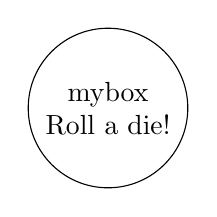
\begin{tikzpicture}
    \node[circle, draw, align=center] {
        \useprotecteddndicon{mybox} \\ 
        Roll a die!
    };
\end{tikzpicture}
\end{codeexample}

% l3draw variant

\RenewCommandCopy\die\DndiconsDie
\RenewCommandCopy\ability\DndiconsAbility

\section[l3draw package variant]{\titlemacro[fontupper=\large\ttfamily]{l3draw} package variant}

A variant of the package that uses the \macro{l3draw} package instead of the \macro{tikz} package is loaded by calling \macro{\usepackage{dndicons-l3draw}} in the preamble of the document after having installed the file \macro{dndicons-l3draw.sty}. The \macro{l3draw} package is an experimental package that provides only basic drawing functionality and therefore loads quicker than Ti*k*Z. The \macro{l3draw} variant thus only supports a certain set of option for styling the icons. 

\begin{macrodef}edge\end{macrodef}
The \macro{l3draw} package is experimental and subject to ongoing updates. Therefore, the \macro{l3draw} variant of the \macro{dndicons} package provides a fallback to established and more stable macro definitions (being available since the last major TeX Live release) which is active per default. Loading the \macro{l3draw} variant of the package with the option \macro{edge} will use functions that are only available in the most recent version of the \macro{l3draw} package.

\label{macro:opacity}
\begin{macrodef}opacity\end{macrodef}
With the \macro{opacity} option, the \macro{l3draw} variant of the \macro{dndicons} package supports transparency using the \macro{l3opacity} package. Since transparency requires management of the PDF settings, it is necessary to call \macro{\DocumentMetadata{}} before loading a \macro{\documentclass}. The \macro{l3opacity} package is experimental.

\subsection{Icon commands}

The commands of the main variant of the \macro{dndicons} package, \macro{\die}, \macro{\ability}, \macro{\saving}, \macro{\spell}, \macro{\spellschool}, \macro{\damage}, \macro{\attack} and \macro{\condition}, which are described above have the same functionality and can be used the same way as in the main variant of the package. However, the available options are different and described in the following in detail.

\begin{macrodef}
|\DndIconsUseIcon|[<options>][<integer>]{<shape>}
|\DndIconsUseIcon*|[<options>][<integer>]{<shape>}
\end{macrodef}
\macro{\DndIconsUseIcon} is the primary command to typeset icons using the \titlemacro{l3draw} variant of the package. The commands \macro{\die}, \macro{\ability}, \macro{\saving}, \macro{\spell}, \macro{\spellschool}, \macro{\damage}, \macro{\attack} and \macro{\condition} are based on this command. 

The \macro{\DndIconsUseIcon} command has a starred version and two optional arguments as well as one mandatory argument. The mandatory argument holds the shape of the icon. All shapes that are described above for the main variant of the package are available. The second optional argument can be used to add an integer when used with shapes for dice.

The starred version of the command is used to fill a frame with color instead of drawing its outline. Frames can be put around the shape via the relevant \macro{frame} option. 

\begin{macrodef}
|\DndiconsDie|[<style>]{<shape>}[<options>]{<integer>}
|\DndiconsAbiliy|[<style>]{<shape>}[<options>]
|\DndiconsSaving|[<style>]{<shape>}[<options>]
|\DndiconsSpell|{<shape>}[<options>]
|\DndiconsSpellschool|[<style>]{<shape>}[<options>]
|\DndiconsDamage|{<shape>}[<options>]
|\DndiconsAttack|{<shape>}[<options>]
|\DndiconsCondition|{<shape>}[<options>]
\end{macrodef}
If that the \macro{dndicons} package is to be loaded together with the \macro{dndicons-l3draw} package or some other package that defines one of the above described basic commands \macro{\die}, \macro{\ability}, \macro{\saving}, \macro{\spell}, \macro{\spellschool}, \macro{\damage}, \macro{\attack} or \macro{\condition}, this set of alternative commands can be used. These commands are exact copies of the relevant basic commands and take the same set or arguments. 

\subsection{Icon options}

\begin{macrodef}
frame
stroke
fill
text
color
background
stroke opacity 
fill opacity
text opacity
opacity 
background opacity
line width
scale
scale inner
rotate
\end{macrodef}
The \macro{\DndIconsUseIcon} command and the commands \macro{\die}, \macro{\ability}, \macro{\saving}, \macro{\spell}, \macro{\spellschool}, \macro{\damage}, \macro{\attack} and \macro{\condition} can be used with certain options that each consist of a key-value pair and can be combined. When used with the \macro{\DndIconsUseIcon} command or the other commands based on this command, these options should be used directly without wrapping them inside the \macro{style} option. 

For example, \macro{\die{eightside}[color=blue, line width=0.8pt]{2}} would result in \die{eightside}[color=blue, line width=0.8pt]{2}.

With the \macro{frame} option, one of four different frames can be selected that are drawn around the shape of the icon. The values \macro{ability} and \macro{damage} draw a circle around the shape. The value \macro{saving} draws a rounded shield and the value \macro{spellschool} draws an angular shield around the shape. The commands \macro{\ability}, \macro{\saving}, \macro{\spellschool} and \macro{\damage} make use of the relevant frame.

The \macro{background} option sets the color of the shape when it is printed over a filled frame which can be achieved by setting the \macro{negative} option for the \macro{\ability} or the \macro{\spellschool} command or using the starred version of the \macro{\DndIconsUseIcon} command.

The \macro{color} option sets the color of strokes, fills and text in general while the \macro{stroke} option, the \macro{fill} option and the \macro{text} option set the color only for strokes, fills or text respectively. Similarly, the \macro{opacity} macro sets the opacity generally, while the options \macro{stroke opacity}, \macro{fill opacity} and \macro{text opacity} allow for setting the opacity of strokes, fill and text separately. The opacity styles are only available when loading the package with the \macro{opacity} option (see the \hyperref{macro:opacity}{description above}). The \macro{line width} sets the line width for strokes. Using the \macro{scale} and \macro{rotate} options, the shape can be scaled and rotated.

The \macro{scale inner} option can be used to change the scaling of the icon when placed inside a frame when using the \macro{\ability}, \macro{\saving}, \macro{\spellschool} and \macro{\damage} macros. The default value is 0.675.

\begin{macrodef}
accessible
accessible = basic
accessible = full
accessible = false
\end{macrodef}
Using the \macro{accessible} option with no value or the value \macro{basic}, a replacement text to the relevant icon can be added which can be copied to the clipboard. The value \macro{full} additionally places an \macro{\Alt} mark in the PDF which means that the shape of the relevant icon is read by screen readers. For this to work, is necessary to call \macro{\DocumentMetadata{}} before loading a \macro{\documentclass}, preferably with tagging enabled to make use of the \macro{accessible} option. The value \macro{full} can be used to disable the function explicitly. Note that depending on the compiler and PDF viewer, there might be line breaks or no spaces before and after the replacement text. 

\begin{macrodef}
every die
every ability
every saving
every spell
every spellschool
every damage
every attack
every condition
every <shape>
\end{macrodef}
Styles following the pattern \macro{dnd icons/every} followed by a space and the name of the command or the shape can be used to apply styles to every instance of this command or shape. For example, \macro{\dndiconsset{every die={color={red}}}} can be used to draw in red all icons created using the \macro{\die} command. Calling \macro{\dndiconsset{every charisma={color={red}}}} will draw every instace of the \macro{charisma} shape in red.

\subsection{Setting options globally}

\begin{macrodef}
|\dndiconsset|
\end{macrodef}
Apart from setting the options to the commands directly, it is also possible to set them globally using the \macro{\dndiconsset} command. Globally set options are overridden by options that are selected directly.

\begin{codeexample}
\dndiconsset{
    color=blue
}

\ability{charisma}
\ability{charisma}[color=red]
\ability{charisma}
\end{codeexample}

\begin{macrodef}
before sep
after sep
baseline
\end{macrodef}
Similar to the settings of the main variant of the package, the spacing before and after the icons can be set using the options \macro{before sep} and \macro{after sep}. The option \macro{baseline} can be used to adjust the baseline of the icons. These options can also be applied to the icon commands directly.

\begin{codeexample}
Roll\die{eightside}{}a die!

\dndiconsset{
    before sep={1cm}
}
Roll\die{eightside}{}a die!
\end{codeexample}

\printchanges

\end{document}

%% End of file `dndicons-doc.tex`.
